
\let\textcircled=\pgftextcircled
\chapter{A brief introduction to Ardupilot}

\initial{A}s it was mentioned in Section \ref{sec:motivation}, it is intended to bring the technology developed within this project to the widest range of UAVs.
However, there exist in the market several families of controller boards (which can be considered to be the brains of the vehicles, in charge of all the basic functions required for an stable flight) that can only be used with specific hardware and/or software, not being compatible with each other since they implement different communication protocols.
Furthermore, some manufacturers work with proprietary software, of which little information on the low-level functioning is available to the public.

It is clearly impractical to try to target all the existing standards for this project, so a compromise needs to be made.
The thesis will be elaborated for the Ardupilot family of controllers, for being the most widespread open-source\footnote{The software is being developed at GitHub: \url{https://github.com/ArduPilot/ardupilot}} alternative.
Some of the leading companies \cite{droneindustryinsights2016} in the sector actively support the Dronecode Project, of which Ardupilot is part, such as Intel, Qualcomm, Parrot, 3DR, Yuneec, AUAV, Walkera\ldots \cite{dronecode2016}

It is important nonetheless to clarify some concepts and features of any Ardupilot-equipped UAV.
More information can be found at \url{www.ardupilot.org}.

\section{Basic features}

The most basic but important feature of the controller is to give control to the pilot over the vehicle.
There are several components that make this function possible.

Firstly, the pilot expresses the desired movements of the vehicle through a Radio Control (RC) transmitter, shown in Figure \ref{fig:RCtransmitter}.
The signal at 2.4 GHz is received by the RC receiver located in the vehicle, depicted in Figure \ref{fig:RCreceiver}.
Then the receiver translates the electromagnetic wave into several PWM (Pulse Width Modulation) signals, one for each input channel up to a maximum of 8 channels, which are inputted to the controller board.
However, for the primary control of the vehicle, only 4 channels are needed: throttle, roll, pitch and yaw.
The additional channels are used to control extra features such as the flight mode, the landing gear or the camera controls.

\begin{figure}[htbp]
	\centering
	\begin{subfigure}[b]{0.25\textwidth}
		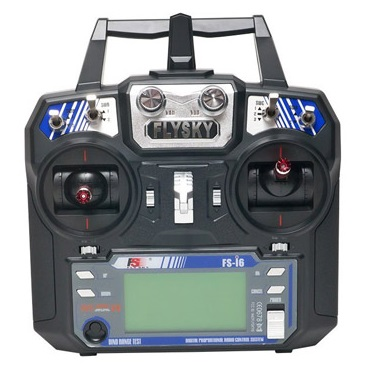
\includegraphics[width=\textwidth]{./figures/RCtransmitter.jpg}
		\caption{RC transmitter}
		\label{fig:RCtransmitter}
	\end{subfigure}
	\hspace{5mm}
	\begin{subfigure}[b]{0.3\textwidth}
		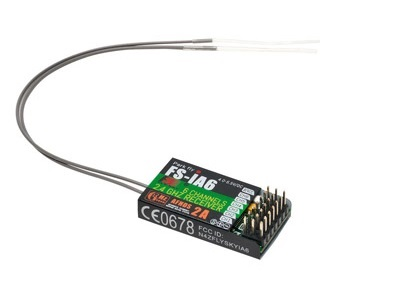
\includegraphics[width=\textwidth]{./figures/RCreceiver.jpg}
		\caption{RC receiver}
		\label{fig:RCreceiver}
	\end{subfigure}
	\caption{FlySky FS-i6 Remote Control (\footnotesize{\url{www.flyskyrc.com}})}
\end{figure}

The second step is to translate the commands from the pilot into signals to the control elements of the vehicle.
These can vary depending on the type of vehicle (for example the yaw command affects the rudder in the case of a fixed-wing aircraft, the tail rotor collective control for a conventional helicopter or the differential throttle in the diagonals for a multicopter) but the underlying processes are similar.

Every Ardupilot controller board must have at least and Inertial Measurement Unit (IMU) consisting of a 3-axis accelerometer plus a 3-axis gyroscope for the state determination of the vehicle.
Additionally, a barometer, a GPS and other sensors can be integrated.
Hence, reading the pilot's commands from the RC receiver and the state of the vehicle from the IMU, the output to the control elements can be computed by some regular PID control loops (more information on the topic can be found at \cite{ogata2010}).
To the output pins of the controller board are connected the control elements, be it some servo-motors for the control surfaces of a fixed-wing aircraft or brushless motors with propellers for the case of a multicopter.
These elements are externally powered by the primary battery.

\section{Ardupilot as part of a UAS}

If Ardupilot wants to be used as a professional tool to enhance production or reduce costs, it can not rely on manual control only. 

\section{Advanced features}


